% DO NOT COMPILE THIS FILE DIRECTLY!
% This is included by the other .tex files.

\begin{frame}[t,plain]
\titlepage
\end{frame}

\section{MISP}

\begin{frame}
    \frametitle{about CIRCL and MISP}
    \begin{itemize}
        \item CIRCL
        \begin{itemize}
            \item National CERT for the private sector, communes, non-govermental entities in Luxembourg
            \item Government-driven initiative, funded by the Ministry of Economy
            \item Mission is to provide a systematic response to computer security threats and incidents
            \item Open Source toolsmiths
        \end{itemize}
        \item Our relationship with MISP has two sides
        \begin{itemize}
            \item We {\bf lead the development} of the MISP platform
            \item We are also involved with and {\bf run several communities}
        \end{itemize}
    \end{itemize}
\end{frame}

\begin{frame}
\frametitle{What is MISP?}
\begin{itemize}
       \item MISP is a {\bf threat information sharing} platform (TISP) built using CakePHP
       \item A tool used and deployed by CSIRTs, SOCs, Cyber threat researchers around the world
       \item Users can either deploy their own MISPs or can become users of an existing MISP instance hosted by someone else
       \item MISP instances can be interconnected, creating large exchange networks with different topologies (mesh, hub/spoke, hybrid)
\end{itemize}
\end{frame}

\begin{frame}
\frametitle{What is the MISP-project?}
\begin{itemize}
        \item Besides being a a web application, the MISP-project also contains the following:
        \begin{itemize}
            \item A set of {\bf open standards} (implemented by MISP and other tools)
            \item An {\bf ecosystem} of libraries, supporting tools
            \item A collection of guidance and best practice documentation by practitioners
        \end{itemize}
        \item All of these are free \& open source
\end{itemize}
\end{frame}

\begin{frame}
\frametitle{What are the objectives of a modern TISP?}      
\begin{itemize}
       \item A tool that {\bf collects threat information} from partners, your analysts, your tools, sensors, feeds
       \item Normalises, {\bf correlates}, {\bf enriches} the data
       \item Manages your processes and automates tasks such as {\bf notifications}, {\bf data flow management}, {\bf triaging} and so on
       \item Allows teams and communities to {\bf collaborate} and rapidly {\bf exchange knowledge}
       \item {\bf Feeds} automated protective tools and analyst tools with the output
       \item {\bf Presents} both individualised and community centric facts, trends, reports of the intelligence
\end{itemize}
\end{frame}


\begin{frame}
 \frametitle{MISP: Started from a practical use-case}
 \begin{itemize}
         \item During a malware analysis workgroup in 2012, we discovered that we worked on the analysis of the same malware.
         \item We wanted to share information in an easy and automated way {\bf to avoid duplication of work}.
         \item Christophe Vandeplas (then working at the CERT for the Belgian MoD) showed us his work on a platform that later became MISP.
         \item A first version of the MISP Platform was used by the MALWG and {\bf the increasing feedback of users} helped us to build an improved platform.
         \item MISP is now {\bf a community-driven development} supporting different intelligence communities.
 \end{itemize}
\end{frame}

\begin{frame}
\frametitle{Development based on practical user feedback}
\begin{itemize}
    \item Organic growth over time within security teams:
        \begin{itemize}
                \item {\bf Malware reversers}: share indicators of analysis with colleagues.
                \item {\bf Security analysts} searching, validating and using indicators in ops.
                \item {\bf Intelligence analysts} researching adversary groups.
                \item {\bf Risk analysis teams} monitoring trends, threats, remediations.
        \end{itemize}
    \item Some examples of other communities picking up MISP:
        \begin{itemize}
                \item {\bf Financial sector}: sharing financial indicators, fraud information.
                \item {\bf Law-enforcement}: bootstrapping DFIR cases, non-cyber-threats, border control, etc
                \item {\bf Military} sharing highly specialised information.
                \item {\bf Disinformation research}: Election interference, disinfo campaigns, etc.
        \end{itemize}
\end{itemize}
\end{frame}

        
\begin{frame}
\frametitle{Why do we develop all of this?}      
\begin{itemize}
   \item {\bf Main goal}: Make our own lives and the lives of our constituency easier
   \begin{itemize}
       \item Our central tool for ingesting, storing and disseminating information...
       \item ...as well as to interact with organisations
       \item By solving issues of other communities, we already have them prepared for information sharing with us when needed
   \end{itemize}
   \item {\bf Secondary}: Democratise threat intelligence for all
   \item {\bf Stretch goal}: Build a full open-source tool-chain for CSIRTs / SoCs / etc
\end{itemize}
\end{frame}

\begin{frame}
 \frametitle{Communities using MISP}
 \begin{itemize}
	 \item Communities are groups of users sharing within a set of common objectives/values.
	 \item CIRCL operates multiple MISP instances with a significant user base (more than 2k organizations with close to 5k users).
         \item {\bf Trust groups} running MISP communities in island mode (air gapped system) or partially connected mode.
	 \item {\bf Financial sector} (banks, ISACs, payment processing organizations) use MISP as a sharing mechanism.
	 \item {\bf Military and international organizations} (NATO, military CSIRTs, n/g CERTs,...).
	 \item {\bf Security vendors} running their own communities.
	 \item {\bf Sectorial communities} Telcoes, ISPs, Medical, ATF, ...
         \item {\bf Topical communities} set up to tackle individual specific issues (disinformation, SIGINT, COVID-19, ...)
 \end{itemize}
\end{frame}


\begin{frame}
\frametitle{Information pipeline}
    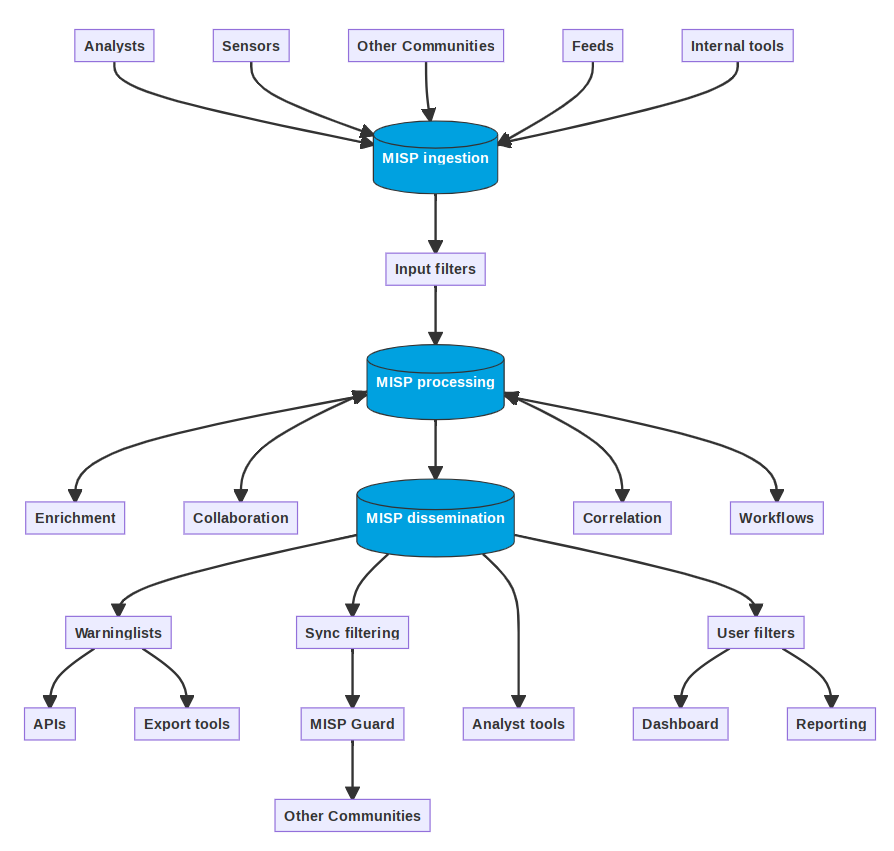
\includegraphics[width=0.75\linewidth]{misp_data_flow.png}
\end{frame}


\section{How can this be relevant to you?}

\begin{frame}
\frametitle{Why should you care?}
    \begin{itemize}
        \item Due to Security
        \begin{itemize}
            \item If you have a security team / operations team looking for threat intel
            \item If you would like to automate your security processes
            \item If you are dealing with security incidents and would like to collaborate
        \end{itemize}
        \item If you're looking for ways to overcome development challenges
        \begin{itemize}
            \item We've been building this by now rather complex application since 2012
            \item Long list of libraries, techniques, ideas that can be reused
        \end{itemize}
        \item Let's dive a bit into the second option and what you'd find in the codebase
    \end{itemize}
\end{frame}

\begin{frame}
\frametitle{Our tech stack}
    \begin{itemize}
        \item Based on CakePHP 2.x, currently being ported to 4.x (5.x once it's out)
        \begin{itemize}
            \item We have a sister project called Cerebrate, which prepared the grounds
            \item CakePHP 4.x based contact management and orchestration platform
        \end{itemize}
        \item MySQL + Redis back-end
        \item Custom front-end using a variety of JS libraries
        \item Different interconnection libraries (Custom, ZMQ, Kafka)
        \item Python module micro-service system built on tornado
        \item Background processing based on Supervisord (previously CakeResque)
    \end{itemize}
\end{frame}

\begin{frame}
\frametitle{Looking for solutions? Some of the issues tackled by MISP:}
    \begin{itemize}
        \item Reusable {\bf libraries} to ease the development (ACL, CRUD, Correlation, etc)
        \item Extensible / customisable data model
        \item Visualisation solutions and dashboarding
    \end{itemize}
    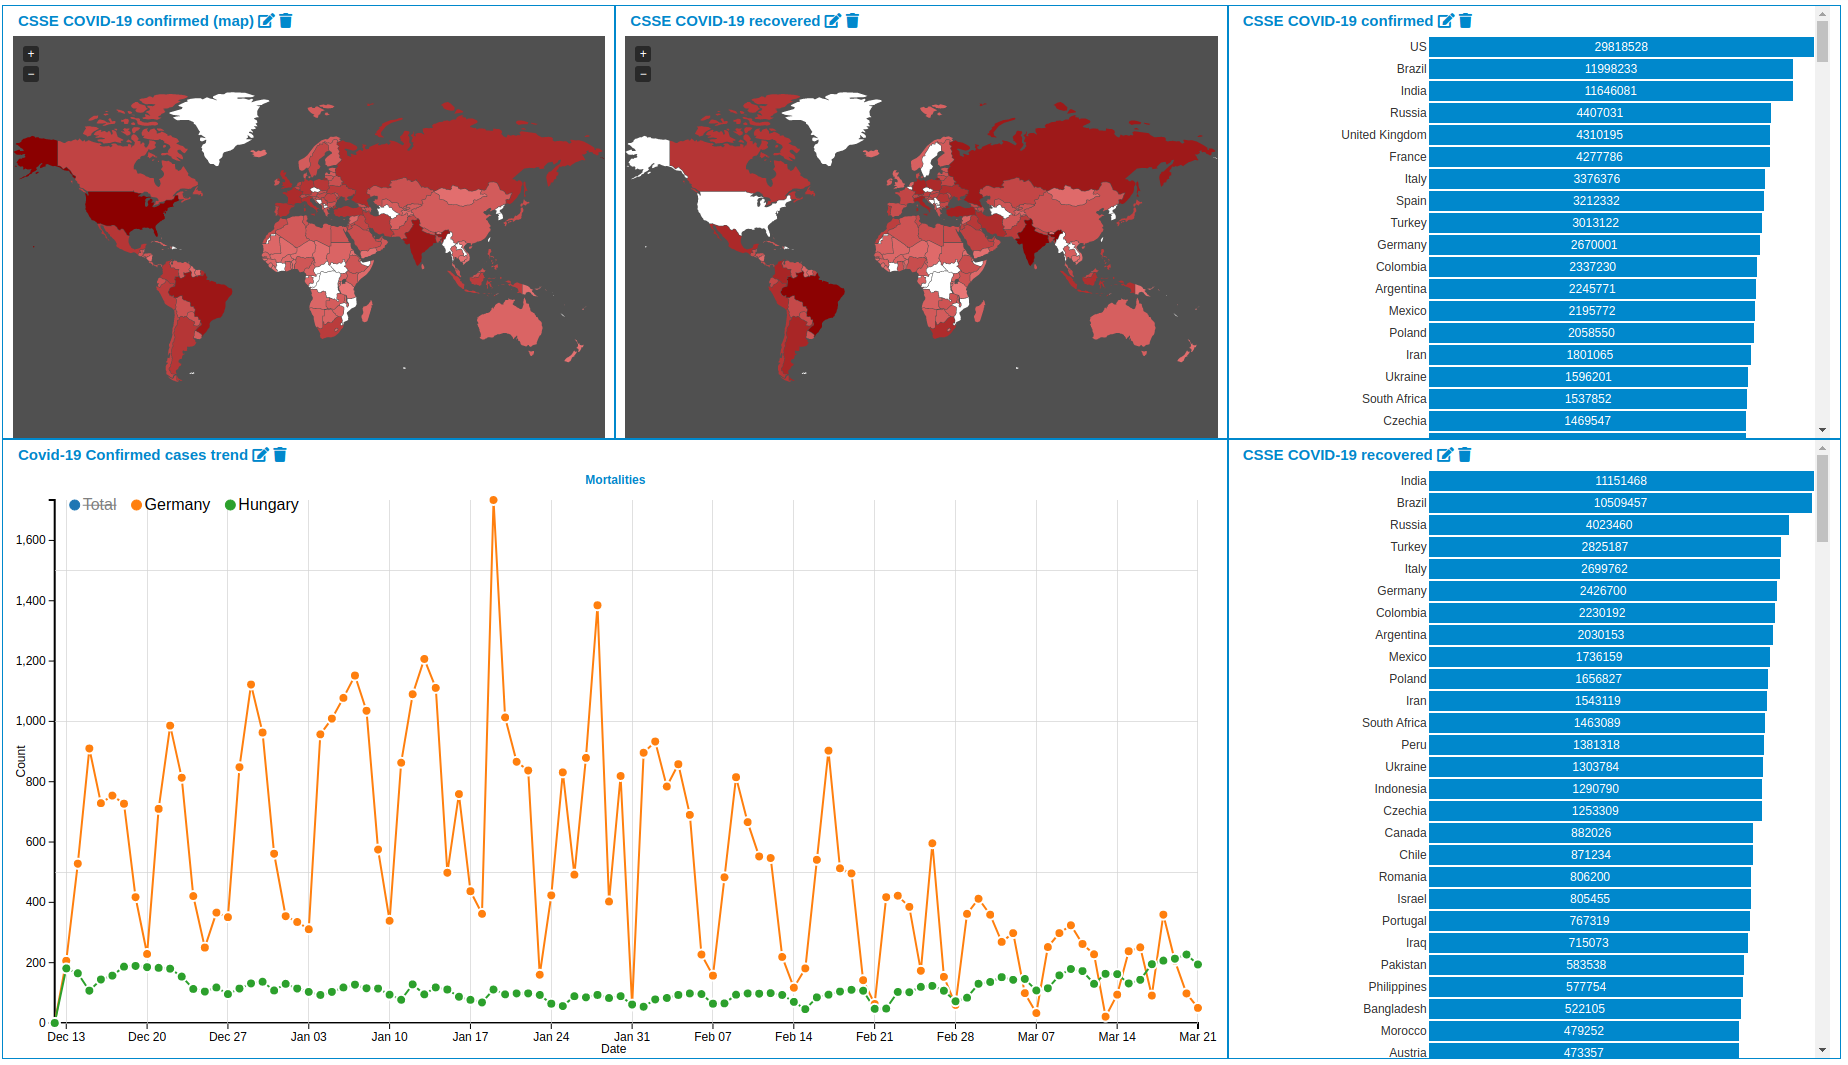
\includegraphics[width=1.00\linewidth]{dashboard.png}
\end{frame}


\begin{frame}
\frametitle{Looking for solutions? Some of the issues tackled by MISP:}
    \begin{itemize}
        \item {\bf UI/API parity} across the entire application
        \item Tight {\bf access control over both data and functionalities}
        \item {\bf Secure information exchange} in adversial conditions
        \begin{itemize}
            \item Cross instance {\bf distribution model}
            \item {\bf Trust group management}
            \item Optional {\bf cryptographic tamper proofing} of data in large mesh networks
        \end{itemize}
    \end{itemize}
    \includegraphics[width=1.00\linewidth]{signed-sync.png}
\end{frame}

\begin{frame}
\frametitle{Looking for solutions? Some of the issues tackled by MISP:}
    \begin{itemize}
        \item Heavy {\bf background processing} and its management
        \item {\bf Communication} via different channels (mailing, different MQs, APIs)
        \item Interactive workflow management
    \end{itemize}
    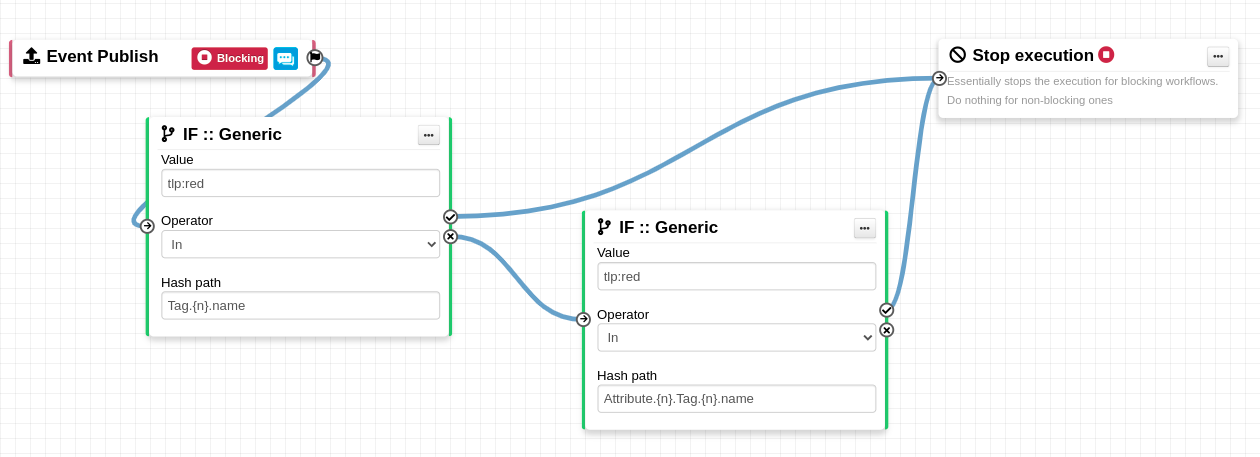
\includegraphics[width=1.00\linewidth]{workflow.png}
\end{frame}

\begin{frame}
\frametitle{Looking for solutions? Some of the issues tackled by MISP:}
    \begin{itemize}
        \item Modular design
        \item Data quality management
        \begin{itemize}
            \item User defined decaying model
            \item False positive management
        \end{itemize}
    \end{itemize}
    \includegraphics[width=1.00\linewidth]{decaying.png}
\end{frame}

\begin{frame}
\frametitle{Quick note about Cerebrate}
    \begin{itemize}
        \item Our CakePHP 4.x based Contact management and Orchestration tool
        \item Large code overlap with MISP (same modular libraries)
        \item Similar design principles
        \item Currently in use at the European CSIRT-Network
        \item Similarly to MISP, OSS
    \end{itemize}
    
\includegraphics[width=1.00\linewidth]{cerebrate.png}
\end{frame}


\begin{frame}
  \frametitle{Get in touch if you have any questions}
  \begin{itemize}
    \item Contact me:
    \begin{itemize}
      \item andras.iklody@circl.lu \url{https://twitter.com/iglocska} \url{https://infosec.exchange/@iglocska}
    \end{itemize}    
    \item Contact us:
    \begin{itemize}
      \item info@circl.lu \url{https://twitter.com/circl_lu} \url{https://www.circl.lu/}
      \item \url{https://github.com/MISP} \url{https://www.misp-project.org/}
      \item \url{https://twitter.com/MISPProject} \url{https://misp-community.org/@misp}
      \item \url{https://github.com/cerebrate-project} \url{https://www.cerebrate-project.org/}
    \end{itemize}
  \end{itemize}
\end{frame}

